%        File: arfc-beamer.tex
%     Created: Sun May 5 10:00 PM 2013 C
%


%\documentclass[11pt,handout]{beamer}
\documentclass[9pt]{beamer}
\usetheme[white]{Illinois}
%\title[short title]{long title}
\title[Short Title]{Synergistic Spent Nuclear Fuel Dynamics Within the European Union}
%\subtitle[short subtitle]{long subtitle}
\subtitle[Short SubTitle]{French Transition into SFRs}
%\author[short name]{long name}
\author[Your Name]{Jin Whan Bae, Kathyrn Huff, Clifford Singer \\ Advanced Reactors and Fuel Cycles Group}
%\date[short date]{long date}
\date[10.22.2017]{October 22, 2017}
%\institution[short name]{long name}
\institute[UIUC]{University of Illinois at Urbana-Champaign}

%%%% Acronym support

\usepackage[acronym,toc]{glossaries}
%\newacronym{<++>}{<++>}{<++>}
\newacronym{ABM}{ABM}{agent-based modeling}
\newacronym{ACDIS}{ACDIS}{Program in Arms Control \& Domestic and International Security}
\newacronym{ADS}{ADS}{Accelerator-Driven Systems}
\newacronym{AHTR}{AHTR}{Advanced High Temperature Reactor}
\newacronym{ANDRA}{ANDRA}{Agence Nationale pour la gestion des D\'echets RAdioactifs, the French National Agency for Radioactive Waste Management}
\newacronym{ANL}{ANL}{Argonne National Laboratory}
\newacronym{ANS}{ANS}{American Nuclear Society}
\newacronym{API}{API}{application programming interface}
\newacronym{ARE}{ARE}{Aircraft Reactor Experiment}
\newacronym{ARFC}{ARFC}{Advanced Reactors and Fuel Cycles}
\newacronym{ASME}{ASME}{American Society of Mechanical Engineers}
\newacronym{ATWS}{ATWS}{Anticipated Transient Without Scram}
\newacronym{BDBE}{BDBE}{Beyond Design Basis Event}
\newacronym{BIDS}{BIDS}{Berkeley Institute for Data Science}
\newacronym{BWR}{BWR}{Boiling Water Reactor}
\newacronym{CAFCA}{CAFCA}{ Code for Advanced Fuel Cycles Assessment }
\newacronym{CDTN}{CDTN}{Centro de Desenvolvimento da Tecnologia Nuclear}
\newacronym{CEA}{CEA}{Commissariat \`a l'\'Energie Atomique et aux \'Energies Alternatives}
\newacronym{CI}{CI}{continuous integration}
\newacronym{CNEN}{CNEN}{Comiss\~{a}o Nacional de Energia Nuclear}
\newacronym{CNERG}{CNERG}{Computational Nuclear Engineering Research Group}
\newacronym{COSI}{COSI}{Commelini-Sicard}
\newacronym{COTS}{COTS}{commercial, off-the-shelf}
\newacronym{CSNF}{CSNF}{commercial spent nuclear fuel}
\newacronym{CTAH}{CTAHs}{Coiled Tube Air Heaters}
\newacronym{CUBIT}{CUBIT}{CUBIT Geometry and Mesh Generation Toolkit}
\newacronym{CURIE}{CURIE}{Centralized Used Fuel Resource for Information Exchange}
\newacronym{DAG}{DAG}{directed acyclic graph}
\newacronym{DANESS}{DANESS}{Dynamic Analysis of Nuclear Energy System Strategies}
\newacronym{DBE}{DBE}{Design Basis Event}
\newacronym{DESAE}{DESAE}{Dynamic Analysis of Nuclear Energy Systems Strategies}
\newacronym{DHS}{DHS}{Department of Homeland Security}
\newacronym{DOE}{DOE}{Department of Energy}
\newacronym{DRACS}{DRACS}{Direct Reactor Auxiliary Cooling System}
\newacronym{DRE}{DRE}{dynamic resource exchange}
\newacronym{DSNF}{DSNF}{DOE spent nuclear fuel}
\newacronym{DYMOND}{DYMOND}{Dynamic Model of Nuclear Development }
\newacronym{EBS}{EBS}{Engineered Barrier System}
\newacronym{EDF}{EDF}{\`{E}lectricit\`{e} de France}
\newacronym{EDZ}{EDZ}{Excavation Disturbed Zone}
\newacronym{EIA}{EIA}{U.S. Energy Information Administration}
\newacronym{EPA}{EPA}{Environmental Protection Agency}
\newacronym{EPR}{EPR}{European Pressurized Reactor}
\newacronym{EP}{EP}{Engineering Physics}
\newacronym{EU}{EU}{European Union}
\newacronym{FCO}{FCO}{Fuel Cycle Options}
\newacronym{FCT}{FCT}{Fuel Cycle Technology}
\newacronym{FEHM}{FEHM}{Finite Element Heat and Mass Transfer}
\newacronym{FEPs}{FEPs}{Features, Events, and Processes}
\newacronym{FHR}{FHR}{Fluoride-Salt-Cooled High-Temperature Reactor}
\newacronym{FLiBe}{FLiBe}{Fluoride-Lithium-Beryllium}
\newacronym{FP}{FP}{Fission Products}
\newacronym{GDSE}{GDSE}{Generic Disposal System Environment}
\newacronym{GDSM}{GDSM}{Generic Disposal System Model}
\newacronym{GENIUSv1}{GENIUSv1}{Global Evaluation of Nuclear Infrastructure Utilization Scenarios, Version 1}
\newacronym{GENIUSv2}{GENIUSv2}{Global Evaluation of Nuclear Infrastructure Utilization Scenarios, Version 2}
\newacronym{GENIUS}{GENIUS}{Global Evaluation of Nuclear Infrastructure Utilization Scenarios}
\newacronym{GPAM}{GPAM}{Generic Performance Assessment Model}
\newacronym{GRSAC}{GRSAC}{Graphite Reactor Severe Accident Code}
\newacronym{GUI}{GUI}{graphical user interface}
\newacronym{HLW}{HLW}{high level waste}
\newacronym{HPC}{HPC}{high-performance computing}
\newacronym{HTC}{HTC}{high-throughput computing}
\newacronym{HTGR}{HTGR}{High Temperature Gas-Cooled Reactor}
\newacronym{IAEA}{IAEA}{International Atomic Energy Agency}
\newacronym{IEMA}{IEMA}{Illinois Emergency Mangament Agency}
\newacronym{IHLRWM}{IHLRWM}{International High Level Radioactive Waste Management}
\newacronym{INL}{INL}{Idaho National Laboratory}
\newacronym{IPRR1}{IRP-R1}{Instituto de Pesquisas Radioativas Reator 1}
\newacronym{IRP}{IRP}{Integrated Research Project}
\newacronym{ISFSI}{ISFSI}{Independent Spent Fuel Storage Installation}
\newacronym{ISRG}{ISRG}{Independent Student Research Group}
\newacronym{JFNK}{JFNK}{Jacobian-Free Newton Krylov}
\newacronym{LANL}{LANL}{Los Alamos National Laboratory}
\newacronym{LBNL}{LBNL}{Lawrence Berkeley National Laboratory}
\newacronym{LCOE}{LCOE}{levelized cost of electricity}
\newacronym{LDRD}{LDRD}{laboratory directed research and development}
\newacronym{LFR}{LFR}{Lead-Cooled Fast Reactor}
\newacronym{LLNL}{LLNL}{Lawrence Livermore National Laboratory}
\newacronym{LMFBR}{LMFBR}{Liquid Metal Fast Breeder Reactor}
\newacronym{LOFC}{LOFC}{Loss of Forced Cooling}
\newacronym{LOHS}{LOHS}{Loss of Heat Sink}
\newacronym{LOLA}{LOLA}{Loss of Large Area}
\newacronym{LP}{LP}{linear program}
\newacronym{LWR}{LWR}{Light Water Reactor}
\newacronym{MAGNOX}{MAGNOX}{Magnesium Alloy Graphie Moderated Gas Cooled Uranium Oxide Reactor}
\newacronym{MA}{MA}{minor actinide}
\newacronym{MCNP}{MCNP}{Monte Carlo N-Particle code}
\newacronym{MILP}{MILP}{mixed-integer linear program}
\newacronym{MIT}{MIT}{the Massachusetts Institute of Technology}
\newacronym{MOAB}{MOAB}{Mesh-Oriented datABase}
\newacronym{MOOSE}{MOOSE}{Multiphysics Object-Oriented Simulation Environment}
\newacronym{MOX}{MOX}{mixed oxide}
\newacronym{MSBR}{MSBR}{Molten Salt Breeder Reactor}
\newacronym{MSRE}{MSRE}{Molten Salt Reactor Experiment}
\newacronym{MSR}{MSR}{Molten Salt Reactor}
\newacronym[longplural={metric tons of heavy metal}]{MTHM}{MTHM}{metric ton of heavy metal}
\newacronym{NAGRA}{NAGRA}{National Cooperative for the Disposal of Radioactive Waste}
\newacronym{NEAMS}{NEAMS}{Nuclear Engineering Advanced Modeling and Simulation}
\newacronym{NEUP}{NEUP}{Nuclear Energy University Programs}
\newacronym{NFCSim}{NFCSim}{Nuclear Fuel Cycle Simulator}
\newacronym{NGNP}{NGNP}{Next Generation Nuclear Plant}
\newacronym{NMWPC}{NMWPC}{Nuclear MW Per Capita}
\newacronym{NNSA}{NNSA}{National Nuclear Security Administration}
\newacronym{NPRE}{NPRE}{Department of Nuclear, Plasma, and Radiological Engineering}
\newacronym{NQA1}{NQA-1}{Nuclear Quality Assurance - 1}
\newacronym{NRC}{NRC}{Nuclear Regulatory Commission}
\newacronym{NSF}{NSF}{National Science Foundation}
\newacronym{NSSC}{NSSC}{Nuclear Science and Security Consortium}
\newacronym{NUWASTE}{NUWASTE}{Nuclear Waste Assessment System for Technical Evaluation}
\newacronym{NWF}{NWF}{Nuclear Waste Fund}
\newacronym{NWTRB}{NWTRB}{Nuclear Waste Technical Review Board}
\newacronym{OCRWM}{OCRWM}{Office of Civilian Radioactive Waste Management}
\newacronym{ORION}{ORION}{ORION}
\newacronym{ORNL}{ORNL}{Oak Ridge National Laboratory}
\newacronym{PARCS}{PARCS}{Purdue Advanced Reactor Core Simulator}
\newacronym{PBAHTR}{PB-AHTR}{Pebble Bed Advanced High Temperature Reactor}
\newacronym{PBFHR}{PB-FHR}{Pebble-Bed Fluoride-Salt-Cooled High-Temperature Reactor}
\newacronym{PEI}{PEI}{Peak Environmental Impact}
\newacronym{PH}{PRONGHORN}{PRONGHORN}
\newacronym{PRIS}{PRIS}{Power Reactor Information System}
\newacronym{PRKE}{PRKE}{Point Reactor Kinetics Equations}
\newacronym{PSPG}{PSPG}{Pressure-Stabilizing/Petrov-Galerkin}
\newacronym{PWAR}{PWAR}{Pratt and Whitney Aircraft REeactor}
\newacronym{PWR}{PWR}{Pressurized Water Reactor}
\newacronym{PyNE}{PyNE}{Python toolkit for Nuclear Engineering}
\newacronym{PyRK}{PyRK}{Python for Reactor Kinetics}
\newacronym{QA}{QA}{quality assurance}
\newacronym{RDD}{RD\&D}{Research Development and Demonstration}
\newacronym{RD}{R\&D}{Research and Development}
\newacronym{RELAP}{RELAP}{Reactor Excursion and Leak Analysis Program}
\newacronym{RIA}{RIA}{Reactivity Insertion Accident}
\newacronym{RIF}{RIF}{Region-Institution-Facility}
\newacronym{SFR}{SFR}{Sodium-Cooled Fast Reactor}
\newacronym{SINDAG}{SINDA{\textbackslash}G}{Systems Improved Numerical Differencing Analyzer $\backslash$ Gaski}
\newacronym{SKB}{SKB}{Svensk K\"{a}rnbr\"{a}nslehantering AB}
\newacronym{SNF}{SNF}{spent nuclear fuel}
\newacronym{SNL}{SNL}{Sandia National Laboratory}
\newacronym{STC}{STC}{specific temperature change}
\newacronym{SUPG}{SUPG}{Streamline-Upwind/Petrov-Galerkin}
\newacronym{SWF}{SWF}{Separations and Waste Forms}
\newacronym{SWU}{SWU}{Separative Work Unit}
\newacronym{ThOX}{ThOX}{thorium oxide}
\newacronym{TRIGA}{TRIGA}{Training Research Isotope General Atomic}
\newacronym{TRISO}{TRISO}{Tristructural Isotropic}
\newacronym{TSM}{TSM}{Total System Model}
\newacronym{TSPA}{TSPA}{Total System Performance Assessment for the Yucca Mountain License Application}
\newacronym{UFD}{UFD}{Used Fuel Disposition}
\newacronym{UML}{UML}{Unified Modeling Language}
\newacronym{UNF}{UNF}{Used Nuclear Fuel}
\newacronym{UOX}{UOX}{uranium oxide}
\newacronym{UQ}{UQ}{uncertainty quantification}
\newacronym{US}{US}{United States}
\newacronym{UW}{UW}{University of Wisconsin}
\newacronym{VISION}{VISION}{the Verifiable Fuel Cycle Simulation Model}
\newacronym{VVER}{VVER}{Voda-Vodyanoi Energetichesky Reaktor (Russian Pressurized Water Reactor)}
\newacronym{VV}{V\&V}{verification and validation}
\newacronym{WIPP}{WIPP}{Waste Isolation Pilot Plant}
\newacronym{YMR}{YMR}{Yucca Mountain Repository Site}


\makeglossaries

%\usepackage{bbding}
\usepackage{amsfonts}
\usepackage{adjustbox}
\usepackage{amsmath}
\usepackage{xspace}
\usepackage{graphicx}
\usepackage{subfigure}
\usepackage{booktabs} % nice rules for tables
\usepackage{microtype} % if using PDF
\usepackage{bigints}
\DeclareMathOperator{\erf}{erf}
%I need some complimentary error funcitons... 
\DeclareMathOperator{\erfc}{erfc}
%page numbers
\setbeamertemplate{footline}[page number]
\setbeamertemplate{caption}[numbered]
%Those icons in the references are terrible looking
\setbeamertemplate{bibliography item}[text]

%try to get rid of header on title page\dots
\makeatletter
    \newenvironment{withoutheadline}{
        \setbeamertemplate{headline}[default]
        \def\beamer@entrycode{\vspace*{-\headheight}}
    }{}
\makeatother


\usepackage{booktabs} % nice rules (thick lines) for tables
\usepackage{microtype} % improves typography for PDF
\usepackage{xspace}

\usepackage{tabularx}
\newcolumntype{b}{X}
\newcolumntype{s}{>{\hsize=.5\hsize}X}
\newcolumntype{m}{>{\hsize=.75\hsize}X}

\newcommand{\SN}{S$_N$}
\renewcommand{\vec}[1]{\bm{#1}} %vector is bold italic
\newcommand{\vd}{\bm{\cdot}} % slightly bold vector dot
\newcommand{\grad}{\vec{\nabla}} % gradient
\newcommand{\ud}{\mathop{}\!\mathrm{d}} % upright derivative symbol
\newcommand{\Cyclus}{\textsc{Cyclus}\xspace}%
\graphicspath{ {images/} }
\usepackage[affil-it]{authblk}
\usepackage{tikz}
\usetikzlibrary{positioning, arrows, decorations, shapes }
\usepackage{cleveref}

\usepackage{datatool}
\begin{document}
%%%%%%%%%%%%%%%%%%%%%%%%%%%%%%%%%%%%%%%%%%%%%%%%%%%%%%%%%%%%%
%% From uw-beamer Here's a handy bit of code to place at 
%% the beginning of your presentation (after \begin{document}):
\newcommand*{\alphabet}{ABCDEFGHIJKLMNOPQRSTUVWXYZabcdefghijklmnopqrstuvwxyz}
\newlength{\highlightheight}
\newlength{\highlightdepth}
\newlength{\highlightmargin}
\setlength{\highlightmargin}{2pt}
\settoheight{\highlightheight}{\alphabet}
\settodepth{\highlightdepth}{\alphabet}
\addtolength{\highlightheight}{\highlightmargin}
\addtolength{\highlightdepth}{\highlightmargin}
\addtolength{\highlightheight}{\highlightdepth}
\newcommand*{\Highlight}{\rlap{\textcolor{HighlightBackground}{\rule[-\highlightdepth]{\linewidth}{\highlightheight}}}}
%%%%%%%%%%%%%%%%%%%%%%%%%%%%%%%%%%%%%%%%%%%%%%%%%%%%%%%%%%%%%
%%--------------------------------%%
\begin{withoutheadline}
\frame{
  \titlepage
}
\end{withoutheadline}

%%--------------------------------%%
\AtBeginSection[]{
\begin{frame}
  \frametitle{Outline}
  \tableofcontents[currentsection]
\end{frame}
}

\section{Background}
\begin{frame}
	\frametitle{Agent-based Framework}
	\begin{itemize}
		\item Cyclus is agent-based, which means it's very modular
		\item User can develop / plug in facilities
			\begin{itemize}
				\item User can `design' their own fuel cycle
				\item Highly customizable
			\end{itemize}
	\end{itemize}
	\begin{figure}[htbp!]
        \begin{center}
                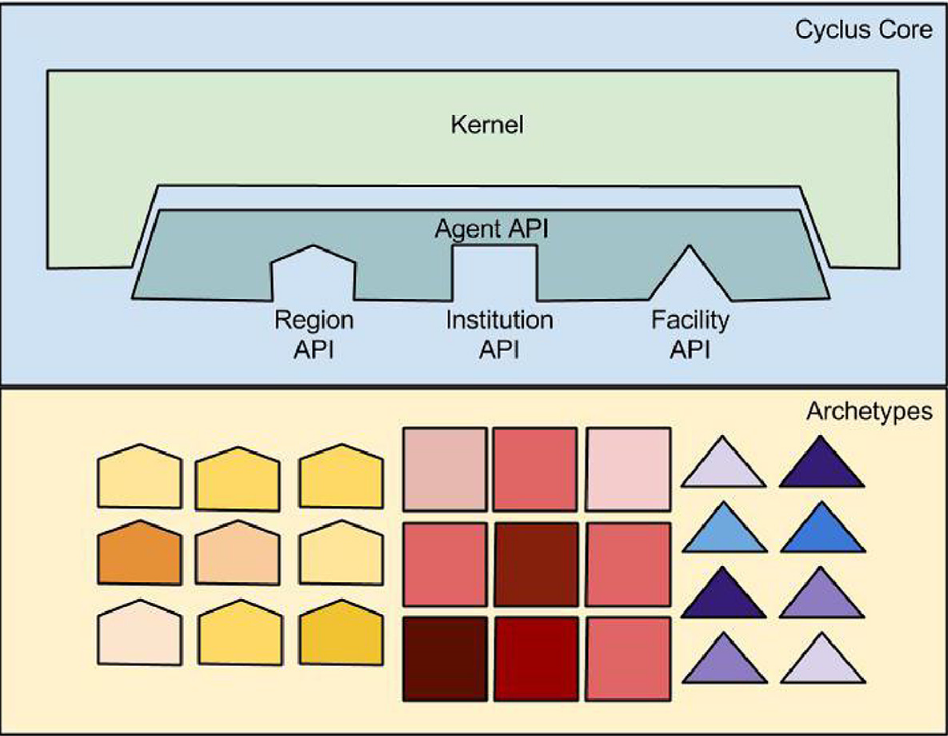
\includegraphics[width=.6\textwidth]{./images/cyclus_structure.png}
        \end{center}
        \caption{Modular Design of Cyclus}
        \label{fig:cyclus_struc}

	\end{figure}
\end{frame}

\begin{frame}
    \frametitle{Timestep Execution}
    A simplified explanation: Each timestep:
    
\begin{figure}[H]
\centering
\begin{tikzpicture}[node distance=1.5cm]
\node (Build) [process] {Build (kernel)};
\node (Tick) [process, below of=Build] {Tick (agent)};
\node (DRE) [process, below of=Tick]{Dynamic Resource Exchange (kernel) };
\node (Tock) [process, below of=DRE]{Tock (agent)};
\node (Decom) [process, below of=Tock] {Decommission (kernel)};

\draw [arrow] (Build) -- (Tick); 
\draw [arrow] (Tick) -- (DRE);
\draw [arrow] (DRE) -- (Tock);
\draw [arrow] (Tock) -- (Decom);
\end{tikzpicture}
\end{figure}

\end{frame}

\begin{frame}
	\frametitle{General Info}
	\begin{itemize}
		\item Written in: C++, Python
		\item Input file: xml, json, python
		\item Output file: .sqlite, .hdf5
	\end{itemize}
\end{frame}


\begin{frame}
	\frametitle{Terminology}
	\begin{itemize}
		\item \textbf{Archetypes}: A collection of logic and behavior which can be configured into a prototype which can then be instantiated in simulation as a agent. Archetypes are represented as C++ classes that inherit from the base cyclus::Agent class. (e.g. Reactor module, Sink module)
		\item \textbf{Prototypes}: Archetype + parameters (e.g. Reactor with input-defined  \texttt{name, cycle time, assembly size, core size etc})
		\item \textbf{Agents}: Every single `entity' in play during simulation (Region, Institution, Facility)
	\end{itemize}
\end{frame}

\begin{frame}
	\frametitle{Terminology}
	\begin{itemize}
		\item \textbf{Region}: The group agent that is a collection of institutions (Can manage / control regions)
		\item \textbf{Institution}: Agent that manages facilities (Can deploy, decommission facilities)
		\item \textbf{Facility}: The agent that `trades' and does calculations (Trades material and transmutes, separates)
	\end{itemize}
\end{frame}

\begin{frame}
	\frametitle{Extensions - Archetypes}
	Since Cyclus is an extensible framework, anyone can develop a new archetype and plug-and-play. (\textcolor{blue}{Institution}, \textcolor{red}{region}, facility otherwise.)
	\begin{itemize}
		\item Cycamore: Sink, Storage, Recipe Reactor, Fuelfab, Enrichment, Source, \textcolor{blue}{DeployInst}, Mixer, Separations, \textcolor{red}{GrowthRegion}
		\item \textcolor{blue}{d3ploy}: Demand-driven deployment Institution (NEUP 16-10512)
		\item CYBORG: Reactor depletion analysis tool using ORIGEN
		\item CYDER: A CYclus Disposal Environment and Repository object.
		\item CORRM: Continuous On-line Reprocessing Reactor Module.
		\item Pyre: Pyroprocessing module with non-proliferation metrics
		\item And more..
	\end{itemize}
\end{frame}

\begin{frame}
	\frametitle{Extensions - Analysis / Drivers}
	There are other tools to help visualization / output data analysis of Cyclus.
	\begin{itemize}
		\item RICKSHAW: Automated stochastic driver for Cyclus
		\item Cymetric: Extracts important fuel cycle metrics
		\item Analysis: Collection of functions to extract metrics (e.g. natU usage, trade between two facilities, etc.)
		\item Cycmap: GIS visualization tool for Cyclus
		\item Cyclist: GUI for Cyclus (DEPRACATED)
	\end{itemize}
\end{frame}


\begin{frame}
	\frametitle{Installation - Binary}
	Better, more thorough explanations are in \texttt{fuelcycle.org}
	\begin{itemize}
		\item Windows: N/A
		\item MacOS: \texttt{conda install -c conda-forge cyclus cycamore}
		\item Linux: \texttt{conda install cyclus cycamore}
	\end{itemize}
\end{frame}


\begin{frame}
	\frametitle{Installation - Build from Source}
    All source files are open-source, and available on Github.

	\texttt{github.com/cyclus/cyclus} and \texttt{github.com/cycamore/cycamore} has the source files, and guides
	\begin{enumerate}
		\item Clone repository (\texttt{git clone [url]})
		\item Install dependency (see github guide README)
		\item \texttt{python install.py}
	\end{enumerate}
\end{frame}


\begin{frame}
	\frametitle{Installation - TroubleShooting}
	Look for your error message or make a new post in the following Cyclus communities:
	\begin{enumerate}
		\item Github Issue in \texttt{github.com/cyclus/cyclus}
		\item Cyclus google user group
        \item Email jbae11@illinois.edu (me)
	\end{enumerate}
\end{frame}



\section{Scenario Specification}
\subsection{Assumptions}

\begin{frame}
	\frametitle{Assumptions}
	\begin{itemize}
		\item Fuel cycle facility parameters (throughput, availability)
		\item Compositions of fresh and spent fuel
		\item Material flow
	\end{itemize}
\end{frame}

\begin{frame}
	\frametitle{Assumptions}
	\begin{itemize}
		\item SFR technology available for deployment in 2040.
		\item Reactor construction is always completed on time.
		\item Separated uranium is unused and stockpiled.
		\item LWRs have a lifetime of 60 years, unless shut down prematurely.
		\item SFRs have a lifetime of 80 years.
	\end{itemize}
	For the French Transition Scenario:
	\begin{itemize}
		\item Reprocessing and fabrication begins 2020
		\item French nuclear capacity remains constant at 66,000 MWe
		\item Reprocessing and fabrication capacity is unlimited.
	\end{itemize}
\end{frame}

%tikz styling definitions

\tikzstyle{decision} = [diamond, draw, fill=blue!20, 
text width=4.5em, text badly centered, node distance=3cm, inner sep=0pt]
\tikzstyle{block} = [rectangle, draw, fill=blue!20, 
text width=5em, text centered, rounded corners, minimum height=4em]
\tikzstyle{line} = [draw, -latex']
\tikzstyle{cloud} = [draw, ellipse,fill=red!20, node distance=3cm,
minimum height=2em]

\subsection{Simulation Parameters}

\begin{frame}
	\frametitle{Material Flow}
	
\begin{figure}
        \begin{adjustbox}{max totalsize={0.9\textwidth}{.8\textheight}, center}
                \begin{tikzpicture}[align=center, node distance = 3cm and 3cm, auto]
                % Place nodes
                \node [block] (sr) {Mine (\texttt{SOURCE})};
                \node [cloud, below of=sr] (nu) {Nat U};
                \node [block, below of=nu] (enr) {Enrichment ({\small \texttt{ENRICHMENT}})};
                \node [cloud, below of=enr] (uox) {\gls{UOX}};
                \node [block, below of=uox] (lwr) {\gls{LWR} (\texttt{REACTOR})};
                \node [cloud, right of=lwr] (snf) {\gls{UNF}};
                \node [block, right of=snf] (pool) {Pool (\texttt{Storage})};
                \node [cloud, left of=lwr] (tl2) {Dep U};
                \node [cloud, right of=enr] (tl) {Dep U};
                \node [block, right of=tl] (sk) {Repository (\texttt{SINK})};
                \node [cloud, below of=sk] (cunf) {Cooled \gls{UNF}};
                \node [cloud, below of=pool] (cunf2) {Cooled \gls{UNF}};
                \node [block, below of=snf] (rep) {Reprocessing ({\small \texttt{SEPARATIONS}})};
                \node [cloud, below of=rep] (u) {Sep. U} ;
                \node [cloud, left of=rep] (pu) {Sep. Pu};
                \node [block, left of=pu] (mix) {Fabrication (\texttt{MIXER})};
                \node [cloud, below of=mix] (mox) {\gls{MOX}};
                \node [block, below of=mox] (mxr) {\gls{MOX} Reactors};
                \node [cloud, right of= mxr] (snmox) {Spent \gls{MOX}};
                
                
                \draw[->, thick] (sr) -- (nu);
                \draw[->, thick] (nu) -- (enr);
                \draw[->, thick] (enr) -- (tl);
                \draw[->, thick] (enr) -- (tl2);
                \draw[->, thick] (tl) -- (sk);
                \draw[->, thick] (tl2) -- (mix);
                \draw[->, thick] (enr) -- (uox);
                \draw[->, thick] (uox) -- (lwr);
                \draw[->, thick] (lwr) -- (snf);
                
                \draw[->, thick] (lwr) -- (snf);
                \draw[->, thick] (snf) -- (pool);
                \draw[->, thick] (pool) -- (cunf);
                \draw[->, thick] (pool) -- (cunf2);
                \draw[->, thick] (cunf) -- (sk);
                \draw[->, thick] (cunf2) -- (rep);
                
                \draw[->, thick] (rep) -- (u);
                \draw[->, thick] (rep) -- (pu);
                \draw[->, thick] (pu) -- (mix);
                \draw[->, thick] (mix) -- (mox);
                \draw[->, thick] (mox) -- (mxr);
                \draw[->, thick] (mxr) -- (snmox);
                \draw[->, thick] (snmox) -- (rep);
                \end{tikzpicture}
                \end{adjustbox}
                
                \caption{Model Fuel Cycle with \gls{MOX} Reprocessing}
                \label{diag:fc}
\end{figure}
\end{frame}

\begin{frame}
	\frametitle{First Simulation - EU Nuclear Opearations \textasciitilde 2050}
	Deployment and Reactor data from \gls{IAEA} \gls{PRIS}.
	Reprocessing plant and fabrication plant modeled after French La Hague and MELOX site
	\cite{schneider_spent_2008, hugelmann_melox_1999}.
		
\begin{table}[h]
	\centering
	\begin{tabularx}{\textwidth}{bb}
		\hline
		Parameter & Value \\
		\hline
		Simulation Start Year & 1970   \\
		Simulation End Year & 2050  \\ 
		Reprocessing Capacity & 91.6 [MTHM \gls{UNF} per month] \cite{schneider_spent_2008}  \\
		Reprocessing Efficiency & 99.8 [\%] \\
		Reprocessing Streams & Plutonium and Uranium  \\
		\gls{MOX} Fabrication & \small{9\% Reprocessed Pu + 91\% Depleted U} \\
		\gls{MOX} Fabrication Throughput & 16.25 [MTHM \gls{MOX} per month]  \cite{hugelmann_melox_1999} \\
		\gls{MOX} Fuel Reprocessing Stage &  Used \gls{MOX} is not reprocessed. \\  
		Reprocessed Uranium Usage &  None. Stockpile reprocessed U \\
		\hline
	\end{tabularx}
	\caption {Parameter for Historical Operation of \gls{EU} Case}
	\label{tab:sim_eu}
\end{table}
	
\end{frame}

\begin{frame}
	\frametitle{Second Simulation - French Transition to SFRs \textasciitilde 2160}
	
\begin{table}[h]
	\centering
	\begin{tabularx}{\textwidth}{bb}
		\hline
		Parameter & Value \\
		\hline
		Simulation Time & 1970-2160 \\
		\gls{SFR} Available Year & 2040 \\
		Reprocessing Capacity & $\infty$ \\
		Reprocessing and Fabrication Begins & 2020 \\
		Separation Efficiency & 99.8 [\%] \\
		Reprocessing Streams & plutonium and uranium \\
		\small{Used \gls{UOX} Inventory} & 144,437 [MTHM] {\small (From first simulation)} \\
		\small{Additional Used \gls{UOX} or Depleted U} & None  \\
		\gls{MOX} Fabrication &  \small{22\% Reprocessed Pu + 78\% Depleted U}  \\
		\gls{MOX} Fabrication Throughput & $\infty$ \\
		\gls{MOX} Fuel Reprocessing Stage &  Used \gls{MOX} gets reprocessed infinitely. \\
		Reprocessed Uranium Usage &  None. Stockpile reprocessed U. \\
		\hline
	\end{tabularx}
	\caption {Parameter for French Transition to \gls{SFR} case }
	\label{tab:sim_france}
\end{table}

\end{frame}


\begin{frame}
	\frametitle{Reactor Parameters - \glspl{LWR} }
	Number of assemblies are linearly adjusted from a model 1,000 MWe reactor.
	\begin{table}[h]
    \centering
    \begin{tabularx}{\textwidth}{bccc}
        \hline
        Parameter & Units & PWR & BWR \\
        \hline
        cycle time & months & \multicolumn{2}{c}{18}   \\ 
        refueling outage & months & \multicolumn{2}{c}{2}\\
        Fuel mass per assembly & kg & 523.4 & 180 \\
        Burnup & GWd/MTHM & \multicolumn{2}{c}{51} \\
        \small{Num. of assem. per core} & (for 1,000 MWe) & 193  & 764 \\
        \small{Num. of assem. per batch} & (for 1,000 MWe) & 62 & 127 \\
        Fuel & & \gls{UOX}, \gls{MOX} & \gls{UOX}  \\
        \hline
    \end{tabularx}
    \caption {\gls{LWR} Parameters}
    \label{tab:lwr}
    \end{table}
\end{frame}


\begin{frame}
	\frametitle{Reactor Parameters - ASTRID-type SFRs}
	
\begin{table}[h]
	\centering
	\begin{tabularx}{\textwidth}{bb}
		\hline
		Parameter & Value \\
		\hline
		SFR Cycle Time & 12 months \\ 
		SFR Refueling Outage & 2 months \\
		Fuel Mass per Batch & 5568 kg \\
        Initial Pu Loading & 4.9 Tons \\
		Batch per Core & 4 \\
		Power Output & 600 MWe \\
		lifetime & 80 years \\
		Fuel & {\small \gls{MOX} (78\% Tailings, 22\% Separated Pu)}\\
		\hline
	\end{tabularx}
	\caption {\gls{SFR} ASTRID Parameters \cite{varaine_pre-conceptual_2012}}
	\label{tab:sfr}
\end{table}
\end{frame}


\section{Future Predictions}
\subsection{Future Projections}

\begin{frame}
	\frametitle{Future Deployment of Reactors in \gls{EU}}
	The power reactors listed in the table are used in the simulation
	to predict \gls{EU} \gls{UNF} inventory in 2050. The table is from
	the World Nuclear Association \cite{world_nuclear_association_nuclear_2017}.
	\begin{table}[h]
	\centering
	\caption {Power Reactors under construction and planned \cite{world_nuclear_association_nuclear_2017}}
	\label{tab:eu_deployment}
	\scalebox{0.70}{
	\begin{tabular}{|c|c|c|c|c|}
		\hline
		Exp. Operational & Country & Reactor & Type & Gross MWe\\
		\hline
		2018 & Slovakia  & Mochovce 3 & PWR & 440\\
		2018 & Slovakia & Mochovce 4 & PWR & 440 \\
		2018 & France & Flamanville 3 & PWR & 1600 \\
		2018 & Finland & Olkilouto 3 & PWR & 1720 \\		
		2019 & Romania & Cernavoda 3 & PHWR & 720 \\
		2020 & Romania & Cernavoda 4 & PHWR & 720 \\
		2024 & Finland & Hanhikivi & VVER1200 & 1200 \\
		2024 & Hungary & Paks 5 & VVER1200 & 1200 \\
		2025 & Hungary & Paks 6 & VVER1200 & 1200 \\
		2025 & Bulgaria & Kozloduy 7 & AP1000? & 950 \\
		2026 & UK & Hinkley Point C1 & EPR & 1670 \\
		2027 & UK & Hinkley Point C2 & EPR & 1670 \\
		2029 & Poland & Choczewo & N/A & 3000 \\
		2035 & Poland & N/A & N/A & 3000 \\
		2035 & Czech Rep & Dukovany 5 & N/A & 1200 \\
		2035 & Czech Rep & Temelin 3 & AP1000 & 1200 \\
		2040 & Czech Rep & Temelin 4 & AP1000 & 1200 \\
		\hline
	\end{tabular}
	}
\end{table}
\end{frame}


\begin{frame}
	\frametitle{Simulated European Deployment}
	
\begin{table}[h]
	\centering
	\begin{adjustbox}{max totalsize={1.1\textwidth}{.8\textheight}, center}
		\begin{tabularx}{\textwidth}{smb}
			\hline 
			
			Nation & Growth Trajectory & Specific Plan \\
			\hline \hline
			UK & Aggressive Growth & 13 units (17,900 MWe) by 2030.\\
			\hline
			Poland & Aggressive Growth & Additional 6,000 MWe by 2035.\\
			\hline
			Hungary & Aggressive Growth & Additional 2,400 MWe (VVER-1200) by 2025. \\ 
			\hline
			Finland & Modest Growth & Additional EPR in 2018, VVER in 2024.\\
			\hline
			Bulgaria & Modest Growth & Additional AP1000 (1,000 MWe) construction in 2035. \\
			\hline
			Romania & Modest Growth & Additional 1,440 MWe by 2020. \\
			\hline
			Czech Rep. & Modest Growth & Additional 2,400 MWe (AP1000s) by 2035.\\
			\hline
			France & Maintenance & Shutdown nuclear plants if they reach end of lifetime. No new construction.\\
			\hline
			Spain & Modest Reduction & No plans to expand or early shutdown. \\
			\hline
			Italy & Modest Reduction & No plans to expand or early shutdown. \\
			\hline
			Belgium & Aggressive Reduction & All shut down 2025.\\
			\hline
			Sweden & Aggressive Reduction & All shut down 2050.\\
			\hline
			Germany & Aggressive Reduction & All shut down by 2022.\\
			\hline
			
		\end{tabularx}
	\end{adjustbox}
	\caption {Future Nuclear Programs of \gls{EU} Nations \cite{world_nuclear_association_nuclear_2017}}
  \label{tab:eu_growth}
\end{table}
\end{frame}



\section{Results}
\subsection{EU Nuclear Operation until 2050}

\begin{frame}
	\frametitle{Historical Operation of EU Reactors}

\begin{table}[h]
	\centering
	\scalebox{0.86}{
		\begin{tabular}{cccc}
			\hline
			\textbf{Category } & \textbf{Value} & \textbf{Unit} & \textbf{Specifics}\\ \hline
			Total UOX Usage  & 176,600 & MTHM &  \\ 
			Total MOX Usage  & 6,953 & MTHM & \\ 
			Total Used UOX Stored  & 110,013 & MTHM & \gls{UNF} that is not reprocessed\\  
			Total Used UOX Stored (France) & 12,943 & MTHM & \gls{UNF} that is not reprocessed \\
			Total Tails  & 1,059,210 & MTHM & \\ 
			Total Natural U Used  & 1,235,810 & MTHM & \\ \hline
		\end{tabular}}
		\caption{Simulation Results for Historical Nuclear Operation 
		of \gls{EU} Nations}
		\label{tab:sim_result}
\end {table}

\end{frame}

\begin{frame}
	\frametitle{Tails and UNF Inventory}
\begin{figure}[htbp!]
\begin{minipage}[b]{.45\linewidth}
	\begin{center}
		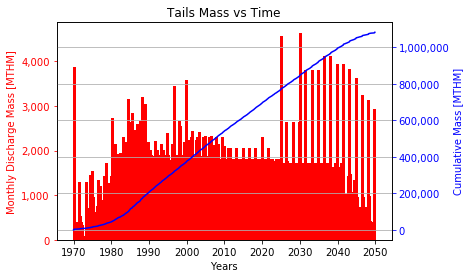
\includegraphics[width=\textwidth]{./images/eu_future/tails.png}
	\end{center}
	\caption{Timeseries of Tails Mass in the \gls{EU}.}
	\label{fig:eu_tail}
\end{minipage}
\hspace{.5cm}
\begin{minipage}[b]{.45\linewidth}
	\centering
	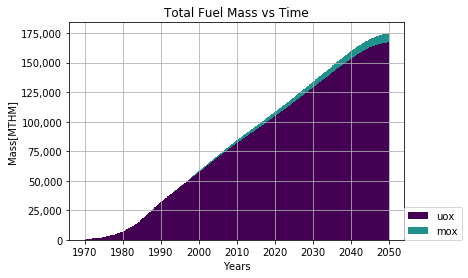
\includegraphics[width=\textwidth]{./images/eu_future/total_fuel.png}
	\caption{Timeseries of Total Fuel Usage in \gls{EU}.}
	\label{fig:eu_fuel}
\end{minipage}
\end{figure}
\end{frame}

\begin{frame}

\begin{figure}[htbp!]
	\begin{center}
			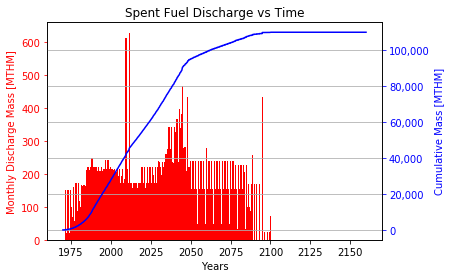
\includegraphics[scale=0.7]{./images/eu_future/snf_discharge.png}
	\end{center}
	\caption{Timeseries of Used Nuclear Fuel in \gls{EU}.}
	\label{fig:eu_snf}
\end{figure}

\end{frame}

\subsection{French Transition Scenario ~2160}

\begin{frame}
	\frametitle{SFR Deployment with Legacy UNF}
	\begin{itemize}
		\item Reprocessing UNF from all EU nations can start approx. 202 SFRs.
		\item Two generations of 66GWe SFRs = 220 SFRs
		\item Breeding Ratio of SFRs over one. ($\frac{23.95}{22.0} = 1.088$)
		\item Initial Pu loading of $4.9$ tons for ASTRID-type SFR \cite{varaine_pre-conceptual_2012}.
		\item $\frac{Pu \ from \ legacy \ \gls{UNF}}{4.9} \approx 202$
	\end{itemize}
\end{frame}

\begin{frame}
	\frametitle{Frech Transition Results}
	
\begin{table}[h]
	\centering
	\scalebox{0.86}{
		\begin{tabular}{ccc}
			\hline
			\textbf{Category} & \textbf{Unit} & \textbf{Value}  \\ \hline
			Total MOX used & MTHM & 63,820  \\ 
			Total \glspl{SFR} Deployed & & 220 \\ 
			Total Plutonium Reprocessed & MTHM & 15,099 \\ 
			Total \gls{ASTRID} fuel from UOX Waste & MTHM & 2,923  \\ 
			Total \gls{ASTRID} fuel from MOX Waste & MTHM  & 60,535 \\ 
			Total Tails used & MTHM & 49,779 \\ 
			Total legacy UNF reprocessed & MTHM & 54,111 \\ 
			Total Reprocessed Uranium Stockpile & MTHM & 183,740 \\ 
			Total Raffinate & MTHM & 33,806 \\ \hline
		\end{tabular}}
		\caption {\gls{SFR} Simulation Results}
		\label{tab:sfr_sim_result}
\end{table}

\end{frame}

\begin{frame}
	\frametitle{Material Flow in French Transition Scenario}
	
\begin{figure}[htbp!]
\begin{minipage}[b]{.45\linewidth}
	\begin{center}
		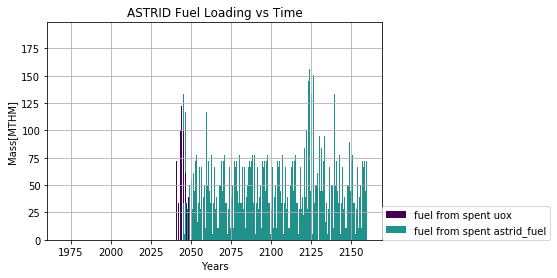
\includegraphics[width=\textwidth]{./images/french-transition/where_fuel.png}
	\end{center}
	\caption{Timeseries of fuel loaded into \glspl{SFR}, separated by origin}
	\label{fig:fuel}
\end{minipage}
\hspace{.5cm}
\begin{minipage}[b]{.45\linewidth}
	\centering
		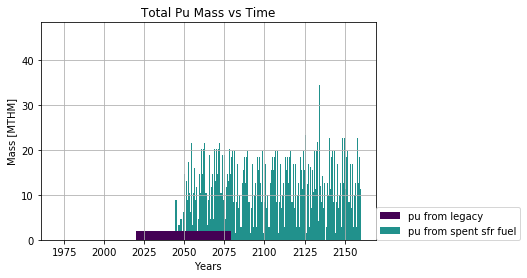
\includegraphics[width=\linewidth]{./images/french-transition/pu.png}
	\caption{Separated plutonium discharge from Reprocessing Plant}
	\label{fig:pu_no_cum}
\end{minipage}
\end{figure}

\end{frame}

\begin{frame}
	\frametitle{Material Flow in French Transition Scenario}
	
\begin{figure}[htbp!]
\begin{minipage}[b]{.45\linewidth}
	\begin{center}
		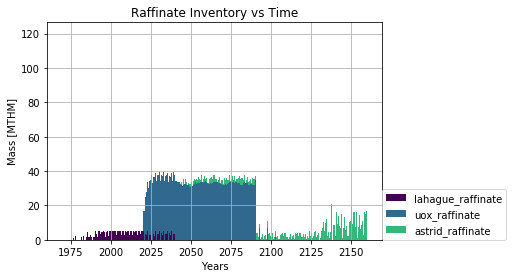
\includegraphics[width=\textwidth]{./images/french-transition/raffinate.png}
	\end{center}
	\caption{Timeseries of raffinate discharge from reprocessing plants}
	\label{fig:fuel}
\end{minipage}
\hspace{.5cm}
\begin{minipage}[b]{.45\linewidth}
	\centering
		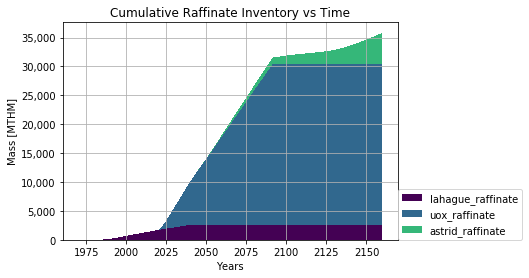
\includegraphics[width=\linewidth]{./images/french-transition/raffinate_cum.png}
	\caption{Cumulative raffinate inventory separated by origin}
	\label{fig:pu_no_cum}
\end{minipage}
\end{figure}

\end{frame}

\section{Conclusion / Discussion}
\begin{frame}
  \frametitle{Conclusions}
        \begin{block}{This study outcomes}
        \begin{itemize}
                \item New tool SaltProc was developed to simulate fuel depletion in the \gls{MSR} core with taking into account online reprocessing.
                \item SaltProc was tested for \gls{MSBR} conceptial design, equilibrium fuel salt composition was found and verified against recent \gls{ORNL} studies.
		\item Average $^{232}$Th refill rate throughout 20 years of operation is approximately 2.39 kg/day or 100 g/GWh$_e$.
		\vspace*{0.15in}
		\item New tool Moltres was developed for modeling coupled physics in fluid-fuelled, molten salt reactors.
		\item The 2D-axisymmetric and 3D multiphysics models are presented.
		\item Moltres demonstrated strong parallel scaling (up to 384 physical cores) on a typical model problem but further optimization required.
		\item Over 55'000 node-hours were consumed on Blue Waters to perform this research.
        \end{itemize}
        \end{block}
        
\end{frame}

\begin{frame}
  \frametitle{Future research}
         
              \begin{block}{Future research effort}
                 \begin{enumerate}
                \item Equilibrium state search for Transatomic \gls{MSR} (\textgreater 30'000 node-hours).
                \item Fuel cycle performance analysis for load-following regime \\ (\textgreater 40'000 node-hours).
                \item \gls{LWR} fuel transmutation in \gls{MSR} viability (\textgreater 30'000 node-hours).
		\vspace*{0.15in}
                \item Start exploring transients in Moltres, e.g. explore responses to reactivity insertion or gaseuos poisons removal (\textgreater 70'000 node-hours).
               \end{enumerate}
               \end{block}
\end{frame}



%%--------------------------------%%
%%--------------------------------%%
\begin{frame}[allowframebreaks]
  \frametitle{References}
  \bibliographystyle{abbrv}
  {\footnotesize \bibliography{bibliography} }
\end{frame}

%%--------------------------------%%


\end{document}



